\documentclass[border=4pt]{standalone}
\usepackage{tikz}
\begin{document}

\noindent
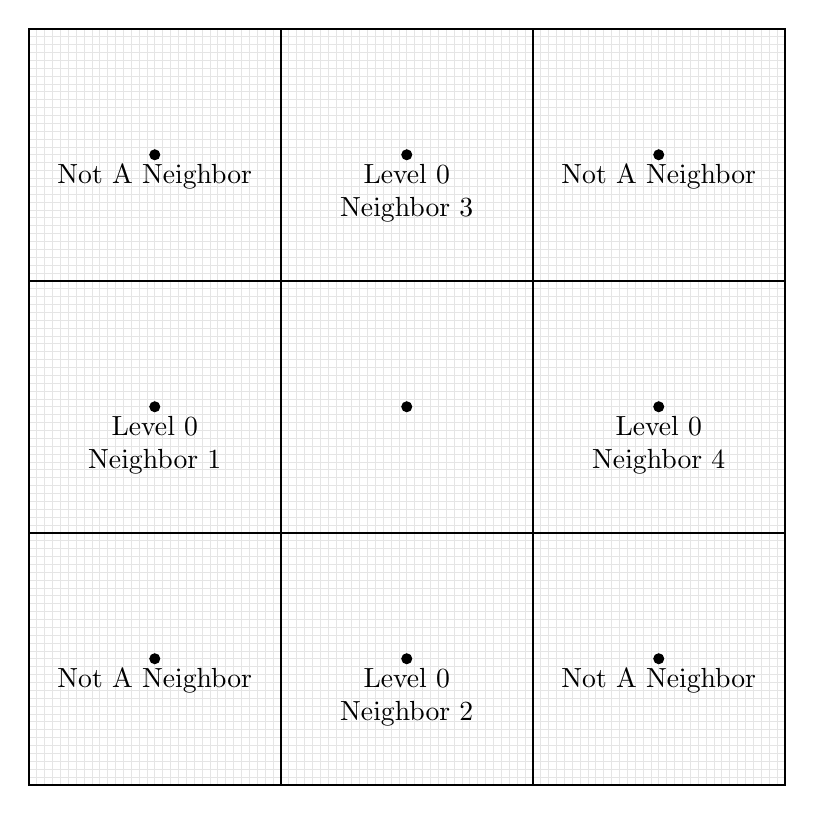
\begin{tikzpicture}[x=0.1cm,y=0.1cm,text centered]

%% (let ((i 0))
%%   (cl-loop for x from 0 upto 2
%%            do (cl-loop for y from 0 upto 2
%%                        do (let* ((xl (* 32 x))
%%                                  (yl (* 32 y))
%%                                  (xu (+ xl 32))
%%                                  (yu (+ yl 32))
%%                                  (xc (+ xl 16))
%%                                  (yc (+ yl 16)))
%%                             (insert (format "\\draw[step=1,black!10,very thin] (%d,%d) grid (%d,%d);\n" xl yl xu yu))
%%                             (insert (format "\\draw[thick] (%d,%d) rectangle (%d,%d);\n" xl yl xu yu))
%%                             (if (or (and (zerop x) (or (zerop y) (= y 2)))
%%                                     (and (= 2 x)   (or (zerop y) (= y 2))))
%%                                 (insert (format "\\node (%03d%03d) at (%d,%d) [below,align=center]  {Not A Neighbor};\n" xc yc xc yc))
%%                                 (if (not (and (= 1 x) (= 1 y)))
%%                                     (progn (cl-incf i)
%%                                            (insert (format "\\node (%03d%03d) at (%d,%d) [below,align=center]  {Level 0\\\\ Neighbor %d};\n" xc yc xc yc i)))))
%%                             (insert (format "\\fill (%d,%d) circle(2pt);\n" xc yc))))))
\draw[step=1,black!10,very thin] (0,0) grid (32,32);
\draw[thick] (0,0) rectangle (32,32);
\node (016016) at (16,16) [below,align=center]  {Not A Neighbor};
\fill (16,16) circle(2pt);
\draw[step=1,black!10,very thin] (0,32) grid (32,64);
\draw[thick] (0,32) rectangle (32,64);
\node (016048) at (16,48) [below,align=center]  {Level 0\\ Neighbor 1};
\fill (16,48) circle(2pt);
\draw[step=1,black!10,very thin] (0,64) grid (32,96);
\draw[thick] (0,64) rectangle (32,96);
\node (016080) at (16,80) [below,align=center]  {Not A Neighbor};
\fill (16,80) circle(2pt);
\draw[step=1,black!10,very thin] (32,0) grid (64,32);
\draw[thick] (32,0) rectangle (64,32);
\node (048016) at (48,16) [below,align=center]  {Level 0\\ Neighbor 2};
\fill (48,16) circle(2pt);
\draw[step=1,black!10,very thin] (32,32) grid (64,64);
\draw[thick] (32,32) rectangle (64,64);
\fill (48,48) circle(2pt);
\draw[step=1,black!10,very thin] (32,64) grid (64,96);
\draw[thick] (32,64) rectangle (64,96);
\node (048080) at (48,80) [below,align=center]  {Level 0\\ Neighbor 3};
\fill (48,80) circle(2pt);
\draw[step=1,black!10,very thin] (64,0) grid (96,32);
\draw[thick] (64,0) rectangle (96,32);
\node (080016) at (80,16) [below,align=center]  {Not A Neighbor};
\fill (80,16) circle(2pt);
\draw[step=1,black!10,very thin] (64,32) grid (96,64);
\draw[thick] (64,32) rectangle (96,64);
\node (080048) at (80,48) [below,align=center]  {Level 0\\ Neighbor 4};
\fill (80,48) circle(2pt);
\draw[step=1,black!10,very thin] (64,64) grid (96,96);
\draw[thick] (64,64) rectangle (96,96);
\node (080080) at (80,80) [below,align=center]  {Not A Neighbor};
\fill (80,80) circle(2pt);




\end{tikzpicture}

\end{document}

